% Provenance (never printed): see sources/outline_sources.md (Year 3:
% sequence stratigraphy, accommodation and supply, systems tracts,
% cyclostratigraphy). Brief: sources/book5/BRIEFS.md, ch. 16. Curves from
% figdata/bachelor-3/shelf_model.py and lr04_periodogram.py. Exercise and
% problem values in the Book 5 scratch calculator calc/ch16.py. The Varden
% basin, its shelf and its core are invented.
\chapter{Sequentiestratigrafie}\label{ch:b3:sequence-stratigraphy}

Over een seismische doorsnede van een continentale marge lopen reflecties aan tegen
oudere, dan bouwen ze uit richting het bekken, daarna trekken ze terug richting het land, en
herhaalt het patroon zich hoger in de reeks. Elk pakket registreert een krachtmeting tussen
twee snelheden: de snelheid waarmee ruimte voor sediment ontstaat, door subsidentie en door
de stijging van de zee, en de snelheid waarmee rivieren die ruimte opvullen.
Sequentiestratigrafie leest de krachtmeting af aan de geometrie van de lagen, en
\omterm{def:b3:sequence-stratigraphy:cyclo}{cyclostratigrafie} leest de klok ervan af aan hun dikte.

\begin{recall}
Accommodatie, eustasie, relatief zeeniveau, subsidentie en het sedimentaire
bekken staan in Boek~3, in het hoofdstuk over diagenese en sedimentaire bekkens.
Uit Boek~4 komen mariene transgressie en regressie en de zeespiegelcyclus van de
eerste orde staan in het hoofdstuk over de fanerozoïsche Aarde; de
Milankovitch-parameters en de klimatologische precessie in het hoofdstuk over orbitale
forcering en de ijstijden; het ouderdomsmodel in het hoofdstuk over klimaatarchieven
en proxy's. \omterm{def:b3:exploration-seismology:terminations}{Onlap}, \omterm{def:b3:exploration-seismology:terminations}{downlap}, \omterm{def:b3:exploration-seismology:terminations}{toplap}, \omterm{def:b3:exploration-seismology:terminations}{erosieve afknotting} en
\omterm{def:b3:exploration-seismology:seismic-stratigraphy}{seismische stratigrafie} staan in Hoofdstuk~\ref{ch:b3:exploration-seismology}. Fourierreeksen
en de Fouriertransformatie staan in de wiskundeboeken.
\end{recall}

\section{Accommodatie, aanvoer en de kustlijn}\label{sec:b3:sequence-stratigraphy:shoreline}

Op elk punt van een bekken stijgt het relatieve zeeniveau met de snelheid $A = \dot E
+ \sigma$, de eustatische snelheid plus de subsidentiesnelheid (een daling bij $A < 0$).
Het relatieve zeeniveau op een plaats wordt bepaald door het mondiale zeeniveau en door
alles wat het land eronder beweegt: \omterm{def:b3:lithosphere-thermal-models:thermal-subsidence}{thermische subsidentie}, de belasting door
het sediment en de buiging die het veroorzaakt, het terugveren van de korst nadat een
ijskap afsmelt, en de trage duw van de mantel onder de plaat. Stijgend
relatief zeeniveau maakt accommodatie; sediment vult die op. Of de
kustlijn zeewaarts of landwaarts beweegt, hangt van beide af en niet
van het zeeniveau alleen.
% ledger: miller20:rsl

\begin{definition}[Normale en geforceerde regressie]\label{def:b3:sequence-stratigraphy:regression}
Een \emph{normale regressie}\index{normale regressie} is een zeewaartse verschuiving van de
kustlijn terwijl het relatieve zeeniveau stijgt: de aanvoer overtreft de
accommodatie die aan de kustlijn ontstaat. Een \emph{geforceerde regressie}\index{geforceerde regressie}
is een zeewaartse verschuiving die wordt aangedreven door een daling van het relatieve zeeniveau: de
kustlijn wordt bekkenwaarts geduwd, ongeacht de aanvoer, en het achtergelaten land
komt bloot te liggen en wordt geërodeerd.
\end{definition}

\begin{definition}[Kustlijntraject]\label{def:b3:sequence-stratigraphy:trajectory}
Het \emph{kustlijntraject}\index{kustlijntraject} is het pad van
de kustlijn door de tijd, getekend in een doorsnede volgens de helling, in het referentiekader van het
sediment, zodat het zowel de horizontale verplaatsing van de kustlijn als de
stijging of daling ten opzichte van de lagen eronder toont.
\end{definition}

Een eenvoudig profiel maakt de krachtmeting exact. Achter de kustlijn ligt een vlakke topset
met breedte $W$ die op zeeniveau ligt; ervoor ligt een foreset met helling
$\tan\theta$ die afloopt naar de bekkenbodem, een hoogte $D$ lager.
De sedimentaanvoer $Q$ is een volume per tijdseenheid per meter kustlijn (een oppervlakte per
tijdseenheid in de doorsnede).

\begin{proposition}[Kustlijntraject]\label{prop:b3:sequence-stratigraphy:trajectory}
Als het relatieve zeeniveau stijgt ($A \ge 0$) en de topset gelijkmatig aggradeert,
beweegt de kustlijn met de snelheid
\[
\frac{\mathrm dx_s}{\mathrm dt} = \frac{Q - AW}{D};
\]
progradeert zolang $Q > AW$ en trekt terug wanneer $AW > Q$. Als het relatieve zeeniveau
daalt ($A < 0$), ontvangt de topset niets en
\[
\frac{\mathrm dx_s}{\mathrm dt} = \frac{Q}{D} + \frac{|A|}{\tan\theta}.
\]
In beide gevallen klimt of daalt het traject onder de hoek waarvan de tangens is
$A/(\mathrm dx_s/\mathrm dt)$.
\end{proposition}

\begin{proof}
In een tijdsinterval $\mathrm dt$ heeft de topset $AW\,\mathrm dt$ aan sediment nodig om
op zeeniveau te blijven. Wat overblijft, $(Q - AW)\,\mathrm dt$, wordt uitgespreid over de foreset,
een wand van hoogte $D$, die vordert met $(Q - AW)\,\mathrm dt/D$; een negatieve
restwaarde betekent dat de zee de topset sneller overstroomt dan dat hij opvult. Als de zee
daalt, ligt de topset boven water en ontvangt niets, en schuift de kustlijn
langs de oude foreset omlaag met $|A|\,\mathrm dt/\tan\theta$ zonder enig
sediment, terwijl de volledige aanvoer de foreset vooruitbouwt met $Q\,\mathrm
dt/D$. De kustlijn stijgt met $A\,\mathrm dt$ ten opzichte van de lagen eronder
terwijl hij met $\mathrm dx_s$ verschuift; daaruit volgt de hoek.
\end{proof}

Een \omterm{def:b3:sequence-stratigraphy:regression}{normale regressie} vraagt daarom een aanvoer die groter is dan de accommodatie
die op de topset ontstaat, en het traject klimt; een \omterm{def:b3:sequence-stratigraphy:regression}{geforceerde regressie} treedt
ongeacht de aanvoer op, en het traject daalt. De verhouding van de twee snelheden,
vaak geschreven als $A/S$, ordent de patronen: progradatie wanneer $A/S < 1$ op de
topset, aggradatie nabij 1, retrogradatie erboven. Dezelfde zeespiegelkromme
kan daardoor een regressie geven op een marge rijk aan sediment en een
transgressie op een sedimentarme.

\section{Stratale geometrie: sequenties en systeemtracten}\label{sec:b3:sequence-stratigraphy:sequences}

De \omterm{def:b3:exploration-seismology:terminations}{reflectiebeëindigingen} van Hoofdstuk~\ref{ch:b3:exploration-seismology}
vormen de woordenschat van de methode: \omterm{def:b3:exploration-seismology:terminations}{onlap} en \omterm{def:b3:exploration-seismology:terminations}{downlap} markeren de basis van een
pakket, \omterm{def:b3:exploration-seismology:terminations}{toplap} en \omterm{def:b3:exploration-seismology:terminations}{erosieve afknotting} de top. Gelezen in een doorsnede volgens de helling, delen ze
een marge op in pakketten begrensd door vlakken van niet-afzetting of
erosie, die elk één cyclus van het relatieve zeeniveau registreren.

\begin{definition}[Afzettingssequentie en sequentiegrens]\label{def:b3:sequence-stratigraphy:sequence}
Een \emph{afzettingssequentie}\index{afzettingssequentie} is een opeenvolging
van genetisch verwante lagen, zonder grote breuk erin, begrensd aan de onderkant
en bovenkant door discordanties of door de conformiteiten die ze in het
bekken voortzetten. Het begrenzende vlak is de \emph{sequentiegrens}\index{sequentiegrens}:
een discordantie, gevormd door blootstelling en erosie op het continentaal plat tijdens een
daling van het relatieve zeeniveau, die bekkenwaarts overgaat
in een correlatieve conformiteit.
\end{definition}

\begin{definition}[Systeemtract]\label{def:b3:sequence-stratigraphy:tract}
Een \emph{systeemtract}\index{systeemtract} is de verzameling van
afzettingssystemen (rivier, kust, plat, helling) die samen actief waren tijdens
één deel van een cyclus van het relatieve zeeniveau, herkenbaar aan zijn positie in de
sequentie, zijn begrenzende vlakken en zijn stapelingspatroon. Er worden vier
onderscheiden:
\begin{itemize}
\item de \emph{systeemtract van de dalende zeespiegel}\index{systeemtract van de dalende zeespiegel},
  opgebouwd door \omterm{def:b3:sequence-stratigraphy:regression}{geforceerde regressie} terwijl het relatieve zeeniveau daalt:
  afbrekende foresets die van het oude plat losraken;
\item de \emph{laagstandsysteemtract}\index{laagstandsysteemtract},
  opgebouwd door \omterm{def:b3:sequence-stratigraphy:regression}{normale regressie} zodra het relatieve zeeniveau weer begint te stijgen,
  op de laagste kustlijnpositie: een wig die aggradeert en progradeert;
\item de \emph{transgressief systeemtract}\index{transgressief systeemtract},
  opgebouwd terwijl de kustlijn landwaarts terugtrekt: terugschrijdende eenheden
  die op het oude plat onlappen;
\item de \emph{hoogstandsysteemtract}\index{hoogstandsysteemtract},
  opgebouwd door \omterm{def:b3:sequence-stratigraphy:regression}{normale regressie} laat in de stijging, wanneer de aanvoer weer sneller is
  dan de accommodatie: foresets die prograderen en downlappen op de afzettingen eronder.
\end{itemize}
\end{definition}

\begin{definition}[Transgressief en maximaal overstromingsvlak]\label{def:b3:sequence-stratigraphy:surfaces}
Het \emph{transgressief vlak}\index{transgressief vlak} is het eerste
significante \omterm{def:b3:sequence-stratigraphy:parasequence}{overstromingsvlak} boven de laagstandafzettingen: het markeert de omslag
van de kustlijn van regressie naar transgressie. Het \emph{maximaal
overstromingsvlak}\index{maximaal overstromingsvlak} markeert de meest landwaartse positie van
de kustlijn, de omslag van transgressie naar hoogstandregressie; de
hoogstand-foresets downlappen erop.
\end{definition}

\begin{definition}[Gecondenseerde sectie en ingesneden dal]\label{def:b3:sequence-stratigraphy:condensed}
Een \emph{gecondenseerde sectie}\index{gecondenseerde sectie} is een dunne laag die
heel langzaam is afgezet ver van de kustlijn, terwijl de zee het plat overstroomt
en het sediment dicht bij de kust wordt vastgehouden: enkele centimeters of decimeters
klei, fossielen, glauconiet of fosfaat die een lange tijd kunnen registreren. Een
\emph{ingesneden dal}\index{ingesneden dal} is een rivierdal dat is ingesneden in het
blootgelegde plat terwijl het relatieve zeeniveau daalt, en dat tijdens de
volgende laagstand en transgressie weer wordt opgevuld.
\end{definition}

\begin{omfigure}
\begin{tikzpicture}[font=\scriptsize, x=0.9cm, y=1.25cm, >=Stealth]
% older highstand deposits below the sequence boundary
\fill[black!10] (0,0) -- (14,0) -- (14,0.4) -- (10,0.6) -- (6,2.8) -- (0,3.0) -- cycle;
\draw[black!35] (1.5,2.0) .. controls (3.2,1.95) and (4.5,1.2) .. (8.5,0.45);
\draw[black!35] (3.5,2.93) .. controls (4.8,2.85) and (6,1.6) .. (10.5,0.42);
% falling-stage systems tract
\fill[red!25] (6.0,2.8) -- (7.4,2.25) -- (8.4,1.85) -- (9.4,1.35) -- (10.4,0.75) -- (10.6,0.58) -- (10,0.6) -- cycle;
\draw[red!60!black] (6.6,2.56) .. controls (7.0,2.4) and (7.5,1.95) .. (8.0,1.70);
\draw[red!60!black] (7.6,2.17) .. controls (8.0,2.0) and (8.5,1.45) .. (9.0,1.15);
\draw[red!60!black] (8.6,1.75) .. controls (9.0,1.55) and (9.5,0.9) .. (10.0,0.6);
% lowstand wedge
\fill[orange!40] (9.2,1.45) -- (10.4,1.5) -- (11.5,1.0) -- (12.6,0.6) -- (13.4,0.44) -- (10.6,0.58) -- (10.4,0.75) -- cycle;
% incised valley and its fill
\fill[orange!30] (2.9,2.9) .. controls (3.3,2.3) and (3.9,2.3) .. (4.3,2.86) -- cycle;
% transgressive systems tract
\fill[green!45!black!35] (11.5,1.0) -- (10.4,1.5) -- (9.2,1.45) -- (8.4,1.85) -- (7.4,2.25) -- (6.0,2.8) -- (1.0,2.97) -- (1.0,3.05) -- (6.0,2.95) -- (7.6,2.5) -- (9.4,1.75) -- (10.8,1.45) -- cycle;
% highstand systems tract
\fill[blue!22] (0,3.62) -- (7.5,3.42) -- (9.8,2.2) -- (11.2,1.22) -- (10.8,1.45) -- (9.4,1.75) -- (7.6,2.5) -- (6.0,2.95) -- (1.0,3.05) -- (0,3.07) -- cycle;
\draw[blue!60!black] (4.0,3.52) .. controls (5.0,3.45) and (5.8,3.1) .. (6.6,2.79);
\draw[blue!60!black] (5.6,3.47) .. controls (6.6,3.4) and (7.4,2.8) .. (8.2,2.26);
\draw[blue!60!black] (6.8,3.44) .. controls (7.8,3.35) and (8.8,2.4) .. (9.7,1.69);
% surfaces
\draw[red!70!black, very thick] (0,3.0) -- (2.9,2.9) .. controls (3.3,2.3) and (3.9,2.3) .. (4.3,2.86) -- (6.0,2.8) -- (7.4,2.25) -- (8.4,1.85) -- (9.2,1.45);
\draw[red!70!black, very thick, densely dashed] (9.2,1.45) -- (9.4,1.35) -- (10.4,0.75) -- (10.6,0.58) -- (14,0.4);
\draw[green!40!black, thick] (11.5,1.0) -- (10.4,1.5) -- (9.2,1.45);
\draw[blue!60!black, thick] (0,3.07) -- (1.0,3.05) -- (6.0,2.95) -- (7.6,2.5) -- (9.4,1.75) -- (10.8,1.45) -- (11.5,1.03) -- (12.6,0.63) -- (13.4,0.47) -- (14,0.43);
% labels
\node[blue!50!black] at (2.6,3.36) {hoogstand (HST)};
\node[green!35!black, anchor=south] at (4.8,3.92) {transgressief (TST)};
\draw[green!35!black] (4.8,3.92) -- (4.4,3.01);
\node[red!60!black, anchor=west] at (10.1,2.45) {dalend zeeniveau (FSST)};
\draw[red!60!black] (10.1,2.45) -- (8.8,1.62);
\node[orange!60!black, anchor=west] at (12.2,1.55) {laagstand (LST)};
\draw[orange!60!black] (12.2,1.55) -- (11.2,0.85);
\node[anchor=north, align=center] at (3.6,2.25) {ingesneden\\ dal};
\node[red!70!black, anchor=north] at (1.4,2.95) {SB};
\node[red!70!black, anchor=north] at (12.0,0.38) {correlatieve conformiteit};
\node[blue!60!black, anchor=west] at (12.7,1.1) {MFS};
\draw[blue!60!black] (12.7,1.1) -- (12.1,0.82);
\node[green!40!black, anchor=west] at (11.6,2.0) {TS};
\draw[green!40!black] (11.6,2.0) -- (10.9,1.27);
\node[blue!60!black, anchor=south] at (13.4,0.58) {gecondenseerd};
\node[anchor=west, black!60] at (0.2,0.35) {oudere afzettingen};
\draw[->] (11.2,3.9) -- (12.6,3.9) node[right] {naar het bekken};
\end{tikzpicture}

\par\smallskip{\small Anatomie van een \omterm{def:b3:sequence-stratigraphy:sequence}{afzettingssequentie} in een helling-doorsnede
(schematisch, verticale schaal sterk overdreven). De \omterm{def:b3:sequence-stratigraphy:sequence}{sequentiegrens} (SB, rood)
is een discordantie op het plat, met een \omterm{def:b3:sequence-stratigraphy:condensed}{ingesneden dal}, en een correlatieve
conformiteit in het bekken (gestippeld); hier is hij getekend boven de
afzettingen van het dalende zeeniveau. Het \omterm{def:b3:sequence-stratigraphy:surfaces}{transgressief vlak} (TS) bedekt de laagstandwig; het
\omterm{def:b3:sequence-stratigraphy:surfaces}{maximaal overstromingsvlak} (MFS) bedekt de dunne transgressieve \omterm{def:b3:sequence-stratigraphy:tract}{systeemtract} en gaat bekkenwaarts
over in een \omterm{def:b3:sequence-stratigraphy:condensed}{gecondenseerde sectie}; de hoogstand-foresets downlappen erop.}\label{fig:b3:sequence-stratigraphy:anatomy}
\end{omfigure}

Waar precies de \omterm{def:b3:sequence-stratigraphy:sequence}{sequentiegrens} in het bekken loopt, is een conventie, en
auteurs verschillen daarin: sommigen tekenen hem aan de basis van de afzettingen van het dalende zeeniveau, waar
de daling begint, anderen aan hun top, waar die eindigt, zoals in de figuur hierboven.
Op het plat is er geen twijfel: de grens is het vlak van blootstelling
en erosie, en de afzettingen erboven zijn jonger dan de daling.

Leest men van onder naar boven op één plek op het buitenste plat, dan registreert een sequentie
de cyclus: hoogstand-foresets, een vlak van blootstelling, mogelijk een dalvulling,
het \omterm{def:b3:sequence-stratigraphy:surfaces}{transgressief vlak}, terugschrijdende lagen, een gecondenseerd interval bij het
\omterm{def:b3:sequence-stratigraphy:surfaces}{maximaal overstromingsvlak}, daarna weer hoogstand-foresets. De hiërarchie van
cycli wordt bepaald door hun oorzaken: het openen en sluiten van oceanen voor de
cyclus van de eerste orde, veranderingen in ijsvolume en in de snelheid van
zeebodemspreiding voor de kortere, en lokale tektoniek en aanvoer voor alle
cycli.

\section{Parasequenties en stapelpatronen}\label{sec:b3:sequence-stratigraphy:parasequences}

Binnen een \omterm{def:b3:sequence-stratigraphy:tract}{systeemtract} zijn de kleinste pakketten die een geoloog op een klif of
in een log kartert, ondiepwordende eenheden van enkele meters tot enkele tientallen
meters dik, afgedekt door een vlak waar plotseling weer dieper water terugkeert.

\begin{definition}[Parasequentie en overstromingsvlak]\label{def:b3:sequence-stratigraphy:parasequence}
Een \emph{parasequentie}\index{parasequentie} is een relatief concordante
opeenvolging van genetisch verwante lagen begrensd door overstromingsvlakken, waarin
het water naar boven toe ondieper wordt: aan een door golven gedomineerde kust gaat slib van de
buitenste kustzone over in onderoever- en bovenoeverzand en strand. Een
\emph{overstromingsvlak}\index{overstromingsvlak} is een vlak waarboven abrupt diepwaterfacies liggen op ondiepere
facies, met aanwijzingen voor een plotselinge verdieping.
\end{definition}

Een enkele \omterm{def:b3:sequence-stratigraphy:parasequence}{parasequentie} wordt naar boven toe grover, en haar gammalog, laag in zand
en hoog in klei, vormt een trechtervorm die naar boven toe smaller wordt. Hoe de
\omterm{def:b3:sequence-stratigraphy:parasequence}{parasequenties} van een tract op elkaar stapelen, vertelt de trend van de
kustlijn: elk daarvan verder zeewaarts opgebouwd dan de vorige (progradationeel),
boven de vorige (aggradationeel), of landwaarts ervan (retrogradationeel). Een log
door de stapel toont de trend rechtstreeks: elke \omterm{def:b3:sequence-stratigraphy:parasequence}{parasequentie} eindigt met
grovere, ondiepere facies dan die eronder, dezelfde, of fijnere en diepere.
Hoogstand- en laagstandtracts stapelen progradationeel of aggradationeel,
transgressieve tracts retrogradationeel. Het volgende hoofdstuk leest zulke logs
facies voor facies.

\begin{omfigure}
\begin{tikzpicture}[font=\scriptsize, x=1cm, y=1cm]
% three logs: each parasequence a coarsening-upward wedge (grain size to the right)
% progradational
\begin{scope}[xshift=0cm]
\fill[yellow!45!brown!35] (0,0) -- (0.5,0) -- (1.4,1.1) -- (0,1.1) -- cycle;
\fill[yellow!45!brown!35] (0,1.1) -- (0.5,1.1) -- (1.8,2.2) -- (0,2.2) -- cycle;
\fill[yellow!45!brown!35] (0,2.2) -- (0.5,2.2) -- (2.2,3.3) -- (0,3.3) -- cycle;
\draw (0,0) -- (0.5,0) -- (1.4,1.1) -- (0.5,1.1) -- (1.8,2.2) -- (0.5,2.2) -- (2.2,3.3) -- (0,3.3) -- cycle;
    \node[anchor=north, align=center] at (1.1,-0.1) {progradationeel\\ (kustlijn beweegt zeewaarts)};
\end{scope}
% aggradational
\begin{scope}[xshift=4.2cm]
\fill[yellow!45!brown!35] (0,0) -- (0.5,0) -- (1.8,1.1) -- (0,1.1) -- cycle;
\fill[yellow!45!brown!35] (0,1.1) -- (0.5,1.1) -- (1.8,2.2) -- (0,2.2) -- cycle;
\fill[yellow!45!brown!35] (0,2.2) -- (0.5,2.2) -- (1.8,3.3) -- (0,3.3) -- cycle;
\draw (0,0) -- (0.5,0) -- (1.8,1.1) -- (0.5,1.1) -- (1.8,2.2) -- (0.5,2.2) -- (1.8,3.3) -- (0,3.3) -- cycle;
    \node[anchor=north, align=center] at (1.1,-0.1) {aggradationeel\\ (kustlijn blijft staan)};
\end{scope}
% retrogradational
\begin{scope}[xshift=8.4cm]
\fill[yellow!45!brown!35] (0,0) -- (0.5,0) -- (2.2,1.1) -- (0,1.1) -- cycle;
\fill[yellow!45!brown!35] (0,1.1) -- (0.5,1.1) -- (1.8,2.2) -- (0,2.2) -- cycle;
\fill[yellow!45!brown!35] (0,2.2) -- (0.5,2.2) -- (1.4,3.3) -- (0,3.3) -- cycle;
\draw (0,0) -- (0.5,0) -- (2.2,1.1) -- (0.5,1.1) -- (1.8,2.2) -- (0.5,2.2) -- (1.4,3.3) -- (0,3.3) -- cycle;
    \node[anchor=north, align=center] at (1.1,-0.1) {retrogradationeel\\ (kustlijn beweegt landwaarts)};
\end{scope}
% flooding surfaces
\foreach \s in {0,4.2,8.4} {
  \draw[omDef, thick] (\s-0.15,1.1) -- (\s+2.5,1.1);
  \draw[omDef, thick] (\s-0.15,2.2) -- (\s+2.5,2.2);
  \node[omDef, anchor=west] at (\s+2.5,1.1) {FS};
  \node[omDef, anchor=west] at (\s+2.5,2.2) {FS};
}
% grain-size axis
\draw[->] (0,3.6) -- (2.3,3.6) node[right] {grover};
\node[anchor=east] at (0,3.6) {modder};
\end{tikzpicture}

\par\smallskip{\small Drie \omterm{def:b3:sequence-stratigraphy:parasequence}{parasequenties}, op drie manieren gestapeld, getekend als
korrelgrootte-logs (breedte naar rechts betekent grover). Elke \omterm{def:b3:sequence-stratigraphy:parasequence}{parasequentie}
wordt naar boven toe grover, van slib van de buitenste kustzone tot onderoeverzand en eindigt bij een
\omterm{def:b3:sequence-stratigraphy:parasequence}{overstromingsvlak} (OV); de top van elk is grover dan die eronder wanneer de stapel
progradeert, gelijk wanneer hij aggradeert, fijner wanneer hij
retrogradeert.}\label{fig:b3:sequence-stratigraphy:stacking}
\end{omfigure}

\begin{inthefield}[Parasequenties in een woestijnklif]
\begin{minipage}[t]{0.52\linewidth}\vspace{0pt}
De Book Cliffs in het oosten van Utah ontsluiten kustafzettingen uit het Boven-Krijt
over tientallen kilometers. In de Kenilworth Member, langs de kliffen gevolgd
van Price tot Hatch Mesa brachten geologen in kaart kustvlakte-, onderwateroever-,
binnenplatform- en ingesneden-dalafzettingen, en negen naar boven grover wordende,
golf- tot stormgedomineerde \omterm{def:b3:sequence-stratigraphy:parasequence}{parasequenties} van 7 tot \qty{32}{m} dik. Naar het bekken toe
splitst elk op in maximaal vier kleinere, naar boven grover wordende laagpakketten van 2 tot
\qty{18}{m} dik; sommige onderwateroeverzanden rusten op een scherpe basis, die de
studie leest als afzettingen van een laagstand.
\end{minipage}\hfill
\begin{minipage}[t]{0.44\linewidth}\vspace{0pt}
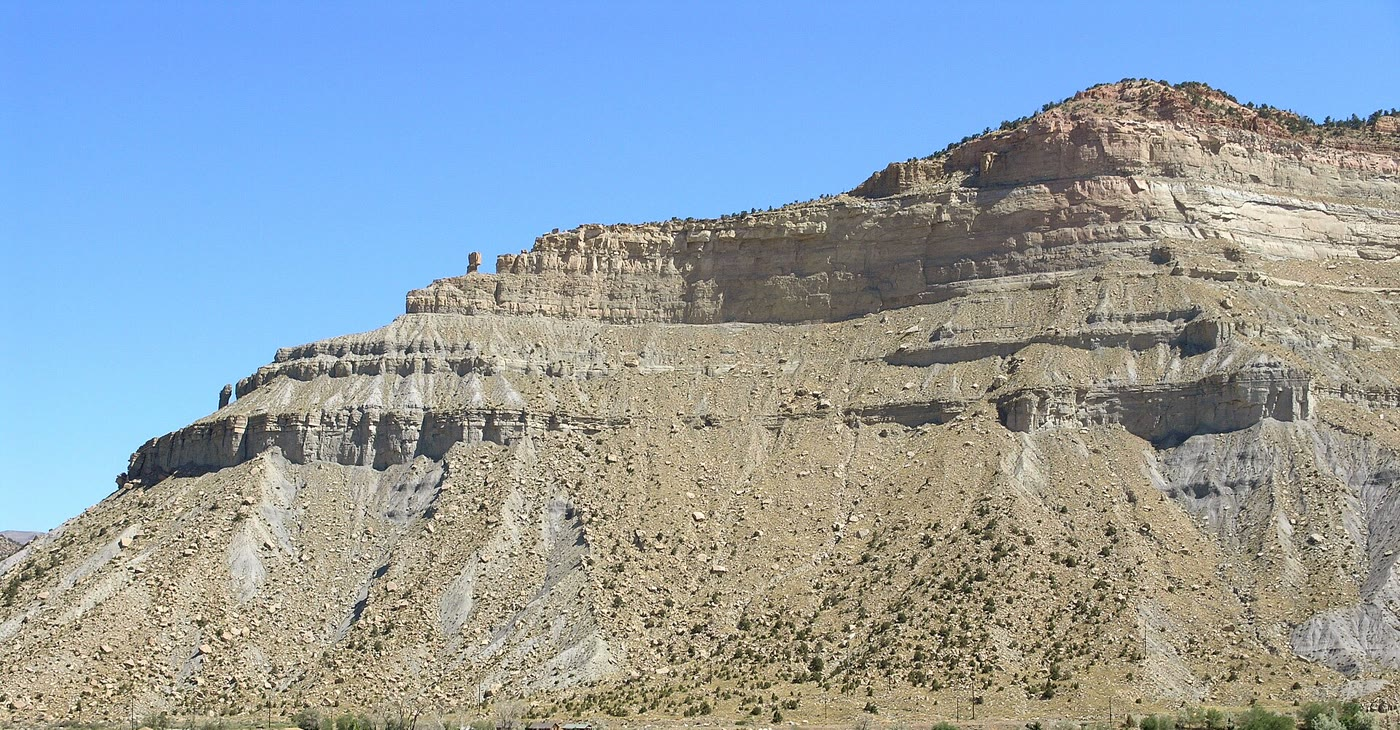
\includegraphics[width=\linewidth]{images/book5/b3-book-cliffs-helper.jpg}

{\scriptsize De Book Cliffs boven Helper, Utah: lichte zandsteenbanken steken
af boven grijze kleisteenhellingen. Foto David Mackie, publiek domein.}
\end{minipage}
\end{inthefield}
% ledger: pattison95:kenilworth, photo:b3-book-cliffs

\section{Een voorwaarts model van een plat}\label{sec:b3:sequence-stratigraphy:model}

De regels van de vorige paragrafen kunnen als model worden doorgerekend. Het Varden-bekken
is een verzonnen plat: een helling die naar het bekken toe afloopt met \qty{1.5}{m/km}, zakkend
met $\sigma = 0.02 + x/1200$ \unit{m/kyr} op een afstand $x$ (km) van het
scharnier, onder een zeeniveau $E = -30\cos(2\pi t/400)$ (m, $t$ in kyr), gevoed door een
rivier die $Q = \qty{6000}{m^3/kyr}$ per meter kust aanvoert. Bij elke stap
van vijfhonderd jaar zakt het bekken; het sediment vult dan een
vlakke topset op tot het zeeniveau, waar het oude oppervlak onder water ligt, en een
foreset met een helling van 0.012 ervoor, de kustlijn zo geplaatst dat het
toegevoegde volume gelijk is aan de aanvoer; blootgesteld land ontvangt niets en, voor
eenvoud, wordt niet geërodeerd. Het model begint in een laagstand, na een eerste
wig die bij constant zeeniveau is opgebouwd.

\begin{omfigure}
\begin{tikzpicture}
\begin{groupplot}[group style={group size=1 by 2, vertical sep=0.35cm, x descriptions at=edge bottom},
  omrecord, width=0.86\linewidth, xmin=0, xmax=600,
  xtick={0,100,200,300,400,500,600},
  tick label style={font=\scriptsize}, label style={font=\small}]
\nextgroupplot[height=0.2\linewidth, ylabel={$E$ (m)}, ymin=-35, ymax=35,
  ytick={-30,0,30}]
\addplot[omDef, thick, domain=0:600, samples=121] {-30*cos(deg(2*pi*x/400))};
\nextgroupplot[height=0.3\linewidth, xlabel={tijd (kyr)}, ylabel={kustlijn $x_s$ (km)},
  ymin=0, ymax=60, ytick={0,20,40,60},
  scatter/classes={1={mark=*, red!70!black}, 2={mark=*, orange!80!black},
    3={mark=*, green!50!black}, 4={mark=*, blue!70!black}}]
% computed in figdata/bachelor-3/shelf_model.py
\addplot[scatter, only marks, mark size=0.9pt, scatter src=explicit symbolic]
  table[x=t, y=xs, meta=tract] {figdata/out/bachelor-3-shelf_model-shore.dat};
\node[font=\scriptsize, orange!60!black] at (axis cs:12,56) {LST};
\node[font=\scriptsize, green!40!black] at (axis cs:70,40) {TST};
\node[font=\scriptsize, blue!60!black] at (axis cs:160,6) {HST};
\node[font=\scriptsize, red!60!black] at (axis cs:300,22) {FSST};
\node[font=\scriptsize, orange!60!black] at (axis cs:415,57) {LST};
\node[font=\scriptsize, green!40!black] at (axis cs:520,45) {TST};
\node[font=\scriptsize, blue!60!black] at (axis cs:580,12) {HST};
\end{groupplot}
\end{tikzpicture}

\par\smallskip{\small Boven, de eustatische zeespiegel van het Varden-model;
onder, de positie van de kustlijn, gekleurd naar \omterm{def:b3:sequence-stratigraphy:tract}{systeemtract} (laagstand
oranje, transgressief groen, hoogstand blauw, dalende fase rood), geclassificeerd
uitsluitend op basis van de uitvoer van het model: dalende fase terwijl de relatieve zeespiegel
bij de kustlijn daalt, transgressief terwijl de kustlijn terugwijkt, laagstand of
hoogstand terwijl hij oprukt onder een stijgende zee, na een daling of na een
transgressie.}\label{fig:b3:sequence-stratigraphy:series}
\end{omfigure}

De figuur hierboven volgt de kustlijn door de tijd, en die hieronder
toont de afzettingen die ze achterliet. De tracten verschijnen zonder dat er
in het model een regel voor is ingebouwd, behalve opvulling en subsidentie. De laagstandskig aan het begin ligt ver
naar buiten; de stijgende zee drijft de kustlijn \qty{38}{km} landwaarts bij de eerste
transgressie, en de hoogstandsforesets bouwen weer naar buiten op zodra de stijging vertraagt.
Dan begint de daling: de kustlijn wordt \qty{33}{km} zeewaarts geduwd in
\qty{187}{kyr}, waarbij dunne, aflopende foresets en een blootgelegd plat achterblijven,
het tract van de dalende fase. Er volgen een nieuwe laagstandskig, een tweede transgressie
en een nieuwe hoogstand. De snelheid van de \omterm{def:b3:sequence-stratigraphy:regression}{geforceerde regressie} in het model
komt binnen enkele procenten overeen met de formule van de propositie; onder een
stijgende zee aggradeert de topset van het model niet uniform, omdat de subsidentie
zeewaarts toeneemt, en de formule is slechts een richtlijn.

\begin{omfigure}
\begin{tikzpicture}
\begin{axis}[omsection, width=0.95\linewidth, height=0.42\linewidth,
  xmin=0, xmax=70, ymin=-150, ymax=40, clip=true,
  xlabel={afstand zeewaarts (km)}, ylabel={hoogte nu (m)},
  xtick={0,10,20,30,40,50,60,70}, ytick={-150,-100,-50,0},
  tick label style={font=\scriptsize}, label style={font=\small}]
% computed in figdata/bachelor-3/shelf_model.py
\addplot[fill=black!10, draw=none] table[x=x, y=z0] {figdata/out/bachelor-3-shelf_model-surfaces.dat} -- (axis cs:120,-300) -- (axis cs:0,-300) -- cycle;
\addplot[fill=orange!45, draw=none] table[x=x, y=z] {figdata/out/bachelor-3-shelf_model-poly1.dat};
\addplot[fill=green!45!black!35, draw=none] table[x=x, y=z] {figdata/out/bachelor-3-shelf_model-poly2.dat};
\addplot[fill=blue!25, draw=none] table[x=x, y=z] {figdata/out/bachelor-3-shelf_model-poly3.dat};
\addplot[fill=red!30, draw=none] table[x=x, y=z] {figdata/out/bachelor-3-shelf_model-poly4.dat};
\addplot[fill=orange!45, draw=none] table[x=x, y=z] {figdata/out/bachelor-3-shelf_model-poly5.dat};
\addplot[fill=green!45!black!35, draw=none] table[x=x, y=z] {figdata/out/bachelor-3-shelf_model-poly6.dat};
\addplot[fill=blue!25, draw=none] table[x=x, y=z] {figdata/out/bachelor-3-shelf_model-poly7.dat};
\addplot[black!45, very thin] table[x=x, y=z40] {figdata/out/bachelor-3-shelf_model-surfaces.dat};
\addplot[black!45, very thin] table[x=x, y=z80] {figdata/out/bachelor-3-shelf_model-surfaces.dat};
\addplot[black!45, very thin] table[x=x, y=z120] {figdata/out/bachelor-3-shelf_model-surfaces.dat};
\addplot[black!45, very thin] table[x=x, y=z160] {figdata/out/bachelor-3-shelf_model-surfaces.dat};
\addplot[black!45, very thin] table[x=x, y=z240] {figdata/out/bachelor-3-shelf_model-surfaces.dat};
\addplot[black!45, very thin] table[x=x, y=z280] {figdata/out/bachelor-3-shelf_model-surfaces.dat};
\addplot[black!45, very thin] table[x=x, y=z320] {figdata/out/bachelor-3-shelf_model-surfaces.dat};
\addplot[black!45, very thin] table[x=x, y=z360] {figdata/out/bachelor-3-shelf_model-surfaces.dat};
\addplot[black!45, very thin] table[x=x, y=z440] {figdata/out/bachelor-3-shelf_model-surfaces.dat};
\addplot[black!45, very thin] table[x=x, y=z480] {figdata/out/bachelor-3-shelf_model-surfaces.dat};
\addplot[black!45, very thin] table[x=x, y=z520] {figdata/out/bachelor-3-shelf_model-surfaces.dat};
\addplot[black!45, very thin] table[x=x, y=z560] {figdata/out/bachelor-3-shelf_model-surfaces.dat};
\addplot[black, thin] table[x=x, y=z600] {figdata/out/bachelor-3-shelf_model-surfaces.dat};
\addplot[black, only marks, mark=*, mark size=0.5pt] table[x=xs, y=zfinal] {figdata/out/bachelor-3-shelf_model-shore.dat};
\node[font=\scriptsize, blue!50!black] at (axis cs:6,4) {HST};
\node[font=\scriptsize, green!30!black] at (axis cs:12,-22) {TST};
\node[font=\scriptsize, red!60!black] at (axis cs:35,-25) {FSST};
\node[font=\scriptsize, orange!60!black] at (axis cs:57.5,-60) {LST};
\node[font=\scriptsize, green!30!black] at (axis cs:36,2) {TST};
\node[font=\scriptsize, blue!50!black] at (axis cs:8,26) {HST};
\end{axis}
\end{tikzpicture}

\par\smallskip{\small Het Varden-plat na \qty{600}{kyr}, in zijn huidige
positie (verticale schaal ongeveer 170 keer overdreven). Kleuren zijn de
\omterm{def:b3:sequence-stratigraphy:tract}{systeemtracten}: laagstand oranje, transgressief groen, hoogstand blauw,
dalende fase rood; grijs is de oudere rampe en de eerste kig. Dunne lijnen zijn
de zeebodem elke \qty{40}{kyr}; zwarte stippen volgen de kustlijn elke
\qty{2}{kyr}. Berekend met het voorwaartse model van de
tekst.}\label{fig:b3:sequence-stratigraphy:section}
\end{omfigure}


De relatieve zeespiegel begint bij de kustlijn te dalen enkele duizenden jaren
na de eustatische hoogstand, omdat eerst de subsidentie moet worden ingehaald,
en hij eindigt enkele duizenden jaren voor de eustatische laagstand. De daling bij
de kustlijn duurt dus minder dan de helft van de eustatische cyclus, en des te
minder naarmate het bekken sneller zakt.

Modellen van dit soort zijn de eerlijke toets van een interpretatie en tonen ook
hun grenzen. Dezelfde sectie kan zijn opgebouwd uit verschillende geschiedenissen: een snellere
daling met minder aanvoer, of een langzamere met meer, of een verandering van subsidentie
in plaats van een verandering van zeespiegel, want de geometrie registreert alleen de relatieve zeespiegel
en de aanvoer. Wereldwijde kaarten van zeespiegelcycli, opgebouwd uit marges in
de jaren 1970 en 1980, leggen de timing vast van veel dalingen die boringen sindsdien
grotendeels hebben bevestigd voor delen van het Laat-Krijt tot het Mioceen, maar hun
amplitudes, zoals een daling van \qty{160}{m} in het midden van het Oligoceen, zijn
een factor 2 tot 3 te hoog. Eustatische amplitudes worden nu afgeleid uit
zuurstofisotopen en uit teruggestripte boringen, en de sequenties van een marge worden
eerst gelezen als een lokaal archief.
% ledger: miller20:epr, miller20:rsl

\section{Cyclostratigrafie}\label{sec:b3:sequence-stratigraphy:cyclo}

Veel sedimentaire opeenvolgingen herhalen zichzelf met regelmatige diktes: paren
van mergel en kalksteen, bundels van vijf paren, grotere sets van bundels. Als
de herhaling wordt bepaald door de Milankovitch-parameters, wordt de dikte van de
cycli tijd.

\begin{definition}[Cyclostratigrafie en astronomische afstemming]\label{def:b3:sequence-stratigraphy:cyclo}
\emph{Cyclostratigrafie}\index{cyclostratigrafie} identificeert en meet
regelmatige cycli in sedimentaire opeenvolgingen en interpreteert ze als registraties van
periodieke forcering, vooral de variaties van de baan en de as van de Aarde.
\emph{Astronomische afstemming}\index{astronomische afstemming} kent ouderdommen toe aan een
opeenvolging door de cycli één voor één af te stemmen op een berekende astronomische
reeks (excentriciteit, obliquiteit, precessie of insolatie), waardoor de cycli worden omgezet in een
ouderdomsmodel.
\end{definition}

De berekende perioden komen uit de oplossing van de beweging van het Zonnestelsel.
De excentriciteit van de baan van de Aarde heeft een hoofdterm van \qty{405}{kyr}, en
vier termen nabij \qty{100}{kyr} (95, 99, 124 en \qty{131}{kyr}); de
obliquiteit een hoofdterm van \qty{41.0}{kyr} met kleinere bij 39.6 en
\qty{53.7}{kyr}. Klimatologische precessie combineert de precessie van de as
met de beweging van het perihelium, bij frequenties $p_0 + g_i$, waarbij $p_0 =
50.47''$ per jaar en de $g_i$ zijn frequenties van de planeetbanen; de
hoofdperioden zijn 23.7, 22.4, 19.1 en \qty{19.0}{kyr}. De term van \qty{405}{kyr}
is de stabielste en dient als metronoom voor oudere opeenvolgingen.
% ledger: la04:eccentricity, la04:obliquity, la04:precession

\begin{omfigure}
\begin{tikzpicture}
\begin{groupplot}[group style={group size=2 by 1, horizontal sep=0.5cm, y descriptions at=edge left},
  omrecord, width=0.52\linewidth, height=0.33\linewidth,
  xmin=0, xmax=0.06, ymin=0, ymax=1.18, clip=false,
  xtick={0,0.02,0.04,0.06}, xticklabels={0,0.02,0.04,0.06}, scaled x ticks=false,
  ytick={0,0.5,1}, title style={font=\small},
  tick label style={font=\scriptsize}, label style={font=\small},
  xlabel={frequentie (cycli per kyr)}]
\nextgroupplot[title={(a) 0 tot \qty{1000}{ka}}, ylabel={relatief vermogen}]
\draw[black!40, densely dotted] (axis cs:0.01,0) -- (axis cs:0.01,1.05);
\draw[black!40, densely dotted] (axis cs:0.0244,0) -- (axis cs:0.0244,1.05);
\draw[black!40, densely dotted] (axis cs:0.0429,0) -- (axis cs:0.0429,1.05);
\draw[black!40, densely dotted] (axis cs:0.0526,0) -- (axis cs:0.0526,1.05);
\node[font=\scriptsize, anchor=south] at (axis cs:0.01,1.05) {100};
\node[font=\scriptsize, anchor=south] at (axis cs:0.0244,1.05) {41};
\node[font=\scriptsize, anchor=south] at (axis cs:0.0429,1.05) {23};
\node[font=\scriptsize, anchor=south] at (axis cs:0.0526,1.05) {19};
% computed in figdata/bachelor-3/lr04_periodogram.py
\addplot[omDef, thick] table[x=f, y=p] {figdata/out/bachelor-3-lr04_periodogram-young.dat};
\nextgroupplot[title={(b) 1250 tot \qty{2500}{ka}}]
\draw[black!40, densely dotted] (axis cs:0.01,0) -- (axis cs:0.01,1.05);
\draw[black!40, densely dotted] (axis cs:0.0244,0) -- (axis cs:0.0244,1.05);
\draw[black!40, densely dotted] (axis cs:0.0429,0) -- (axis cs:0.0429,1.05);
\draw[black!40, densely dotted] (axis cs:0.0526,0) -- (axis cs:0.0526,1.05);
\node[font=\scriptsize, anchor=south] at (axis cs:0.01,1.05) {100};
\node[font=\scriptsize, anchor=south] at (axis cs:0.0244,1.05) {41};
\node[font=\scriptsize, anchor=south] at (axis cs:0.0429,1.05) {23};
\node[font=\scriptsize, anchor=south] at (axis cs:0.0526,1.05) {19};
\addplot[omDef, thick] table[x=f, y=p] {figdata/out/bachelor-3-lr04_periodogram-old.dat};
\end{groupplot}
\end{tikzpicture}

\par\smallskip{\small Periodogrammen van de benthische zuurstofisotopenstapel LR04
in twee vensters (getrend, Hann-taper, genormaliseerd op de grootste piek);
stippellijnen markeren perioden van 100, 41, 23 en \qty{19}{kyr}. (a) De laatste
miljoen jaar: de \qty{100}{kyr}-band domineert. (b) Van 2.5 tot
\qty{1.25}{Ma}: de \qty{41}{kyr}-obliquiteit domineert.}\label{fig:b3:sequence-stratigraphy:periodogram}
\end{omfigure}
% ledger: data:lr04, lr04:tuning

\begin{definition}[Periodogram]\label{def:b3:sequence-stratigraphy:periodogram}
Het \emph{periodogram}\index{periodogram} van een reeks $y_0, \dots, y_{N-1}$
bemonsterd met een stap $\Delta$ (in tijd of diepte), na verwijdering van zijn gemiddelde
en trend en vermenigvuldiging met een taper $w_k$, is
\[
P(f_j) = \Bigl|\sum_{k=0}^{N-1} w_k y_k\, e^{-2\pi i f_j k\Delta}\Bigr|^2,
\qquad f_j = \frac{j}{N\Delta},\ j = 1, \dots, \frac N2:
\]
de vermogensdichtheid van de reeks bij elke frequentie $f_j$, het kwadraat van de modulus van
de discrete Fouriertransformatie ervan.
\end{definition}

Twee getallen bepalen wat een \omterm{def:b3:sequence-stratigraphy:periodogram}{periodogram} kan zien. De frequentiestap, $1/(N\Delta)$,
het omgekeerde van de lengte van de meetreeks, is de resolutie: twee perioden waarvan de
frequenties minder dan dat verschillen, kunnen niet worden gescheiden. De hoogste frequentie, de
Nyquistfrequentie $1/(2\Delta)$, wordt bereikt bij twee monsters per cyclus; een
kortere cyclus gaat niet verloren maar wordt teruggevouwen tot een valse langere. De taper,
hier een Hann-venster, vlakt de uiteinden van de reeks af, zodat een sterke piek
geen vermogen over het hele spectrum lekt.


De periodogrammen hierboven vormen het uitgewerkte voorbeeld. In de laatste miljoen jaar valt de
sterkste piek in de \qty{100}{kyr}-band (bij \qty{91}{kyr} op het frequentieraster
van een meetreeks van \qty{1000}{kyr}, waarvan de buren 100 en \qty{83}{kyr} zijn),
de obliquiteit heeft een derde van zijn vermogen en de precessie enkele procenten;
tussen 2.5 en \qty{1.25}{Ma} draagt de obliquiteit de reeks en
heeft de \qty{100}{kyr}-band een zesde van zijn vermogen. Eén voorbehoud zit in de
gegevens ingebouwd: de LR04-tijdschaal zelf is verkregen door de stapel af te stemmen op een
eenvoudig ijsmodel aangedreven door zomerinsolatie op \ang{65}\,NB, beperkt door gestapelde
sedimentatiesnelheden om overafstemming te voorkomen, dus het vinden van baanperioden daarin is
deels circulair. De toets die niet circulair is, is die in diepte gedaan, vóór enige
afstemming: als de verhoudingen van de dikten van de cycli overeenkomen met de
verhoudingen van de baanperioden, is de forcering aangetoond, en geven de dikten de
sedimentatiesnelheid.
% ledger: lr04:tuning, la04:obliquity

\begin{method}[Sedimentatiesnelheid uit cyclusdikte]\label{met:b3:sequence-stratigraphy:cycles}
\begin{enumerate}
\item bereken het \omterm{def:b3:sequence-stratigraphy:periodogram}{periodogram} van de reeks in diepte, met zijn resolutie
  $1/L$ voor een sectie van lengte $L$ en zijn Nyquistgrens $1/(2\Delta z)$;
\item lijst de golflengten van de significante pieken, $\lambda = 1/f$;
\item vergelijk hun verhoudingen met die van de baanperioden (405 : 100 : 41
  : 23, of 21 voor een gemiddelde precessie); een overeenkomst van drie pieken is een sterk
  argument, één piek alleen geen;
\item deel elke golflengte door zijn periode: de quotiënten, die overeen zouden moeten komen,
  geven de sedimentatiesnelheid.
\end{enumerate}
\end{method}

Een zo verkregen sedimentatiesnelheid is een gemiddelde over de cyclus en
veronderstelt een constante snelheid: een verandering van snelheid binnen de sectie rekt de
pieken uit, en een hiaat verwijdert cycli ongemerkt. Lange opeenvolgingen worden daarom
cyclus voor cyclus afgestemd op de berekende reeks, eerst de \qty{405}{kyr}-cyclus,
en gecontroleerd aan radiometrische ouderdommen waar vulkanische lagen dat toelaten.

\section{Oefeningen}

\begin{exercise}[$\star$]\label{exo:b3:sequence-stratigraphy:1}
Op een punt van een plat shelf stijgt het eustatische zeeniveau met \qty{0.5}{m/kyr} en
zakt het bekken met \qty{0.1}{m/kyr}. Bereken de snelheid van de relatieve
zeespiegelstijging en de accommodatie die in \qty{20}{kyr} ontstaat. Wat is de relatieve
snelheid als de zee in plaats daarvan met \qty{0.3}{m/kyr} daalt?
\end{exercise}

\begin{exercise}[$\star$]\label{exo:b3:sequence-stratigraphy:2}
Benoem voor elk geval het \omterm{def:b3:sequence-stratigraphy:tract}{systeemtract} dat wordt opgebouwd: (a) het relatieve zeeniveau
daalt, de kustlijn beweegt naar zee toe; (b) het relatieve zeeniveau stijgt, de
kustlijn beweegt landwaarts; (c) het relatieve zeeniveau stijgt laat in een
cyclus langzaam, de kustlijn beweegt naar zee toe en de foresets downlappen op een
\omterm{def:b3:sequence-stratigraphy:surfaces}{maximaal overstromingsvlak}; (d) het relatieve zeeniveau is net begonnen te stijgen na een
daling, en de kustlijn beweegt nog steeds naar zee toe.
\end{exercise}

\begin{exercise}[$\star$]\label{exo:b3:sequence-stratigraphy:3}
Een putlog toont drie \omterm{def:b3:sequence-stratigraphy:parasequence}{parasequenties}, die elk naar boven grover worden. De toppen van
de drie, van onder naar boven, zijn fijn zand, middelgrof zand en grof zand met
strandlaminatie. Benoem het stapelingspatroon, de beweging van de kustlijn en de
\omterm{def:b3:sequence-stratigraphy:tract}{systeemtracten} waartoe het kan behoren. Wat zou de omgekeerde volgorde betekenen?
\end{exercise}

\begin{exercise}[$\star$]\label{exo:b3:sequence-stratigraphy:4}
Een klif toont koppels van mergel en kalksteen, gegroepeerd in bundels van vijf; een
bundel is \qty{1.6}{m} dik. Interpreteer de koppels en de bundels met de
baanperiodes, en bereken de sedimentatiesnelheid uit de bundels.
\end{exercise}

\begin{exercise}[$\star\star$]\label{exo:b3:sequence-stratigraphy:5}
Een shelf heeft een topset van \qty{20}{km} breed, een foreset van \qty{50}{m} hoog en een
aanvoer van \qty{4000}{m^3/kyr} per meter kust; het relatieve zeeniveau stijgt
met \qty{0.15}{m/kyr}. Bereken de snelheid van de kustlijn. Met welke
stijgsnelheid zou zij stilstaan?
\end{exercise}

\begin{exercise}[$\star\star$]\label{exo:b3:sequence-stratigraphy:6}
Hetzelfde shelf ziet nu zijn relatieve zeeniveau dalen met \qty{0.2}{m/kyr}; de
helling van de foreset is 0.01. Bereken de snelheid van de \omterm{def:b3:sequence-stratigraphy:regression}{geforceerde regressie} en het
aandeel daarvan dat uitsluitend door de daling wordt veroorzaakt.
\end{exercise}

\begin{exercise}[$\star\star$]\label{exo:b3:sequence-stratigraphy:7}
Het relatieve zeeniveau stijgt met \qty{0.4}{m/kyr} over een topset van \qty{25}{km} breed.
Onder welke aanvoer trekt de kustlijn zich terug? Bij een aanvoer van
\qty{6000}{m^3/kyr} per meter en een onderwateroever van slechts \qty{10}{m} hoog, hoe
snel trekt zij zich terug?
\end{exercise}

\begin{exercise}[$\star\star$]\label{exo:b3:sequence-stratigraphy:8}
De excentriciteitstermen van 94.9 en \qty{123.9}{kyr}, en die van 94.9 en
\qty{98.9}{kyr}: hoe lang moet een reeks zijn om elk paar in een
\omterm{def:b3:sequence-stratigraphy:periodogram}{periodogram} te scheiden? Kan dat met een reeks van \qty{600}{kyr}?
\end{exercise}
% ledger: la04:eccentricity

\begin{exercise}[$\star\star$]\label{exo:b3:sequence-stratigraphy:9}
In een kern beslaan 20 obliquiteitscycli (elk \qty{40.98}{kyr})
\qty{16.4}{m}. Bereken de sedimentatiesnelheid en de tijd tussen twee aslagen die
\qty{3.1}{m} uit elkaar liggen in hetzelfde interval.
\end{exercise}
% ledger: la04:obliquity

\begin{exercise}[$\star\star\star$]\label{exo:b3:sequence-stratigraphy:10}
Bereken de hoek van de kustlijntrajectorie (a) bij een \omterm{def:b3:sequence-stratigraphy:regression}{geforceerde regressie} bij
\qty{200}{m/kyr} met een relatief zeeniveau dat daalt met \qty{0.4}{m/kyr}, (b) bij
een \omterm{def:b3:sequence-stratigraphy:regression}{normale regressie} bij \qty{50}{m/kyr} met een relatief zeeniveau dat stijgt met
\qty{0.2}{m/kyr}. Waarom is een hoek van enkele tienden van een graad makkelijk te zien op een
seismische sectie en moeilijk op een klif?
\end{exercise}

\begin{exercise}[$\star\star\star$]\label{exo:b3:sequence-stratigraphy:11}
De precessieconstante is $p_0 = 50.467718''$ per jaar en vier planetaire
frequenties zijn $g_5 = 4.257564$, $g_2 = 7.456665$, $g_4 = 17.910194$ en
$g_3 = 17.366595''$ per jaar. Bereken de perioden van de klimatologische precessie
$1\,296\,000''/(p_0 + g_i)$. Controleer dat $g_2 - g_5$ en $g_4 - g_5$ de
excentriciteitstermen van 405 en \qty{95}{kyr} geven.
\end{exercise}
% ledger: la04:precession, la04:eccentricity

\begin{exercise}[$\star\star\star$]\label{exo:b3:sequence-stratigraphy:12}
Twee bekkens leggen dezelfde relatieve zeeniveaustijging vast van \qty{0.3}{m/kyr} gedurende
\qty{100}{kyr}. In het eerste bekken stijgt de eustatische zeespiegel met \qty{0.25}{m/kyr} en
zakt het bekken met \qty{0.05}{m/kyr}; in het tweede stijgt de eustatische zeespiegel met
\qty{0.1}{m/kyr} en zakt het bekken met \qty{0.2}{m/kyr}. Toon aan dat de
twee secties identiek kunnen zijn. Welke extra waarneming scheidt de twee
geschiedenissen?
\end{exercise}

\section{Probleem: Zeeniveaus van het Varden-bekken}

\begin{problem}[{Weekendprobleem --- accommodatie, de kustlijntrajectorie en de
systeemtracten van het Varden-shelfmodel, en de klok van een kern}]
\label{pb:b3:sequence-stratigraphy:1}
Het Varden-shelf uit het hoofdstuk zakt met $\sigma = 0.02 + x/1200$
(\unit{m/kyr}, $x$ in km), onder een zeeniveau $E = -30\cos(2\pi t/400)$ (m,
$t$ in kyr), met een aanvoer van \qty{6000}{m^3/kyr} per meter kust en een
helling van de foreset van 0.012. Het model geeft, elke \qty{50}{kyr}, het zeeniveau
$E$, de positie van de kustlijn $x_s$, de snelheid van de relatieve zeeniveaustijging aan de
kustlijn $A$ en de hoogte $D$ van de foreset:

\begin{center}\small
\begin{tabular}{rrrrr|rrrrr}
$t$ & $E$ & $x_s$ & $A$ & $D$ & $t$ & $E$ & $x_s$ & $A$ & $D$\\
(kyr) & (m) & (km) & (m/kyr) & (m) & (kyr) & (m) & (km) & (m/kyr) & (m)\\\hline
50 & $-21.2$ & 33.5 & 0.381 & -- & 350 & $-21.2$ & 44.6 & $-0.276$ & 25.3\\
100 & 0.0 & 15.7 & 0.504 & -- & 400 & $-30.0$ & 51.3 & 0.063 & 81.6\\
150 & 21.2 & 12.8 & 0.364 & 21.1 & 450 & $-21.2$ & 52.7 & 0.397 & 99.2\\
200 & 30.0 & 16.8 & 0.034 & 41.1 & 500 & 0.0 & 40.4 & 0.525 & --\\
250 & 21.2 & 24.0 & $-0.293$ & 45.4 & 550 & 21.2 & 22.9 & 0.372 & --\\
300 & 0.0 & 32.9 & $-0.424$ & 35.7 & 600 & 30.0 & 28.2 & 0.043 & 13.4\\
\end{tabular}
\end{center}
(Een streepje geeft een kustlijn aan die terugtrekt over een vlakke kustvlakte, waar
geen foreset wordt opgebouwd.)

\medskip\noindent\textbf{Deel I --- Accommodatie.}
\begin{enumerate}
\item Bereken de grootste eustatische snelheid en wanneer die optreedt.
\item Bereken de subsidentiesnelheid bij het scharnier, bij 20 en \qty{50}{km}, en
  aan de rand van het model, \qty{120}{km}.
\item De kustlijn staat bij het hoogstand op ongeveer \qty{17.5}{km}. Wanneer begint
  het relatieve zeeniveau daar te dalen?
\item Bij het laagstand bereikt de kustlijn ongeveer \qty{50}{km}. Wanneer houdt
  het relatieve zeeniveau daar op met dalen?
\item Hoe lang duurt de relatieve daling aan de kustlijn, vergeleken met de
  \qty{200}{kyr} van de eustatische daling? Waarom is zij korter?
\item Hoeveel accommodatie maakt subsidentie alleen in één cyclus bij
  \qty{30}{km}? Vergelijk die met de eustatische amplitude.
\end{enumerate}

\medskip\noindent\textbf{Deel II --- De kustlijn.}
\begin{enumerate}[resume]
\item Lees de tabel: tussen welke tijdstippen beweegt de kustlijn zich zeewaarts,
  en tussen welke landwaarts?
\item Een topset van \qty{15}{km} breed bij de hoogstand aggradeert met \qty{0.30}{m/kyr}
  voor een foreset van \qty{40}{m} hoog. Bereken de snelheid van de
  kustlijn met de propositie van het hoofdstuk.
\item Bij welke stijgingssnelheid zou de kustlijn op die topset stoppen met verplaatsen?
\item Bereken op \qty{300}{kyr} de snelheid van de \omterm{def:b3:sequence-stratigraphy:regression}{geforceerde regressie}
  uit de tabel. Het model geeft \qty{204}{m/kyr}: vergelijk.
\item Welke van de twee termen domineert, de aanvoer of de daling?
\item Het traject daalt van \qty{16.3}{m} op \qty{17.4}{km}
  (\qty{204.5}{kyr}) naar \qty{-42.7}{m} op \qty{50.7}{km}
  (\qty{391.5}{kyr}), in huidige hoogten. Bereken de gemiddelde helling ervan.
  Verklaar uit de subsidentie die elk punt sindsdien heeft ondergaan waarom de daling
  bijna gelijk is aan de eustatische daling van \qty{59.7}{m}.
\end{enumerate}

\medskip\noindent\textbf{Deel III --- De systeemtracts.}
\begin{enumerate}[resume]
\item Ken uit de tabel aan elk tijdstip van 150 tot
  \qty{600}{kyr} een \omterm{def:b3:sequence-stratigraphy:tract}{systeemtract} toe.
\item Het model legt het begin van de dalende fase op \qty{204.5}{kyr}
  en het einde ervan op \qty{391.5}{kyr}: controleer die tegen vraag 3 en 4.
\item Waar vormt zich in dit model de \omterm{def:b3:sequence-stratigraphy:sequence}{sequentiegrens}, op het plat en in het bekken?
  Het model erodeert niet: wat zou een echt plat laten zien?
\item De tweede transgressie eindigt op \qty{559}{kyr} met de kustlijn op
  \qty{18.5}{km}. Bereken haar gemiddelde snelheid vanaf haar begin op \qty{52.8}{km} op
  \qty{439.5}{kyr}. Welk vlak vormt zich aan het eind?
\item Waarom is het transgressieve \omterm{def:b3:sequence-stratigraphy:tract}{systeemtract} dun op het plat, en waar zou zich
  een \omterm{def:b3:sequence-stratigraphy:condensed}{gecondenseerde sectie} vormen?
\end{enumerate}

\medskip\noindent\textbf{Deel IV --- Een boorkern uit het bekken.} Een boorkern
\qty{30}{m} lang, om de centimeter bemonsterd, toont een regelmatige
afwisseling; het \omterm{def:b3:sequence-stratigraphy:periodogram}{periodogram} in diepte heeft pieken bij golflengten van 7.5,
2.0 en \qty{0.81}{m}, de grootste bij \qty{2.0}{m}.
\begin{enumerate}[resume]
\item Bereken de frequentieresolutie en de Nyquistfrequentie van het
  \omterm{def:b3:sequence-stratigraphy:periodogram}{periodogram}.
\item Bereken de verhoudingen van de drie golflengten tot de grootste piek, en
  vergelijk ze met de orbitale perioden.
\item Ken aan de pieken perioden toe en bereken uit elk de sedimentatiesnelheid.
  Waarom wijkt de langste enigszins af?
\item Hoe lang beslaat de boorkern?
\item Bij welke golflengte zou de precessie van \qty{23.7}{kyr} moeten verschijnen?
  Kan een boorkern die om de \qty{25}{cm} is bemonsterd hem zien, en waar zou hij vallen?
\item Waarom is een overeenkomst van drie pieken een sterker argument dan één?
\item Geef de maximale verschuiving van de kustlijn in het model naar het bekken toe,
  van het begin van de daling tot het einde van de laagstandregressie.
\end{enumerate}
\end{problem}
% ledger: la04:eccentricity, la04:obliquity, la04:precession
